\RequirePackage{ifpdf}
\documentclass[letterpaper,landscape]{slides}
%\documentclass[letterpaper,portrait]{slides}
\usepackage{boxedminipage}
\usepackage{amsmath}
\usepackage{amssymb}

%\input /u/rhl/TeX/pdf.tex
\input pdf.tex

\newif\ifTalk\Talktrue		% We generating a talk, not printing
%\Talkfalse			% no; we're really printing

%\pagestyle{empty}
\setlength{\topmargin}{-1in}
\setlength{\textheight}{7.5in}
\setlength{\textwidth}{9in}
\setlength{\oddsidemargin}{0pt}
\setlength{\oddsidemargin}{0pt}

%\onlyslides{1-3,4,10-9999}
%\onlyslides{26-9999}

\begin{document}

\newcommand{\XXX}[1]{\textbf{XXX} #1}
\newcommand{\colour}[1]{\color{#1}}

\def\eq#1{\begin{equation} \color{blue} #1 \end{equation}}
\def\vx{{\bf x}}
\def\vv{{\bf v}}
\def\p{\partial}
\def\b#1{{\bf  #1}}
\def\p{\partial}
\def\th{^{th}}
\def\msun{{\rm\,M_\odot}}
\def\bnabla{{\bf\nabla}}
\def\dint{\int\!\!\!\int}
\def\d{{\rm d}}
\def\i{{\rm i}}
\def\ddt#1{{\rm{d} #1\over {\rm dt}}}
\def\ddtS#1{{\rm{d^2} #1\over {\rm dt^2}}}
%\lta and \gta produce > and < signs with twiddle underneath
\def\spose#1{\hbox to 0pt{#1\hss}}
\def\lta{\mathrel{\spose{\lower 3pt\hbox{$\mathchar"218$}}
     \raise 2.0pt\hbox{$\mathchar"13C$}}}
\def\gta{\mathrel{\spose{\lower 3pt\hbox{$\mathchar"218$}}
     \raise 2.0pt\hbox{$\mathchar"13E$}}}
\def\mspace{\hbox{\quad}}
\def\deffn#1{{\bf#1}}\def\eqs#1{equations \rf#1}






\newcount\itemCnt\itemCnt=0
\newcommand{\nitem}{%
  \global\advance\itemCnt by 1
  ~\vskip0cm\the\itemCnt.\qquad}

\definecolor{orange}{rgb}{1.0, 0.5, 0.0}
\definecolor{purple}{cmyk}{0.4, 0.8, 0.3, 0.0}


%%%%%%%%%%%%%%%%%%%%%%%%%%%%%%%%%%%
\newcommand{\onepic}[6]{%
\begin{slide}
     \begin{center}
        \begin{minipage}{#1in}
            {\large \color{blue} #6}
            \phantom{x} \vskip #2in
            \phantom{x} \hskip #3in
            {\scalebox{#4}{\includegraphics{#5}}}   
        \end{minipage}
     \end{center}
    \vfill
\end{slide}
}


%%%%%%%%%%%%%%%%%%%%%%%%%%%%%%%%%%%
\newcommand{\picslide}[7]{%
  \begin{slide}
     \begin{center}
        \begin{minipage}{#5in}
            \hskip #6in
            \hskip -1in
            {\scalebox{#4}{\includegraphics{#1.#2}}}
            \vskip #7in~
            {\large \color{blue} #3}
        \end{minipage}
     \end{center}
     \vfill
  \end{slide}
}
%%%%%%%%%%%%%%%%%%%%%%%%%%%%%%%%%%%
 

%%%%%%%%%%%%%%%%%%%%%%%%%%%%%%%%%%%
\newcommand{\Spicslide}[7]{%
  \begin{slide}
     \begin{center}
        \begin{minipage}{#5in}
            \vskip #6in
            \hskip #7in
            {\scalebox{#4}{\includegraphics{#1.#2}}}
        \end{minipage}
     \end{center}
     \vfill
  \end{slide}
}
%%%%%%%%%%%%%%%%%%%%%%%%%%%%%%%%%%%
 



%------------------------------------------------------------------------------

\begin{slide}

\phantom{x}
\vskip -2in
\begin{center}
\bfseries
{\large {\color{blue} Astr 511: Galaxies as galaxies}}
\end{center}

{\centerline {{\color{blue} 
Winter Quarter 2017, University of Washington}}}
{\centerline {{\color{blue} 
Mario Juri\'{c} \& \v{Z}eljko Ivezi\'{c} }}}

\vskip 1.6in

{\centerline {\Large {\color{red}      Lecture 8:             }}}
\vskip 0.2in 
{\centerline {\huge {\color{blue} Dynamics III: Building }}}
\vskip 0.1in
{\centerline {\huge {\color{blue} Galaxy Models }}}

\vfill
\end{slide}
%------------------------------------------------------------------------------


%------------------------------------------------------------------------------
\begin{slide}
\vskip 4.5in
\begin{center}
{\large \color{red} 
                  Using the CBE to Build Galaxy Models   }
\end{center}

\vskip 3.8in

\begin{flushright}
{ \tiny - Binney \& Tremaine, \S4. } \\
\vskip 0.5em
{ \tiny - Barnes, Galaxies, \url{https://www.ifa.hawaii.edu/~barnes/ast626_09/scbe.pdf} }
\end{flushright}

\end{slide}


%------------------------------------------------------------------------------
\begin{slide}
\begin{center}
{\large \color{red} 
                  Integrals of Motion   }
\end{center}

An {\bf integral of motion} is any function $I({\bf r}, {\bf v})$ of the
phase space coordinates $({\bf r}, {\bf v})$ that satisfies:

\eq{
	\frac{d}{dt}I({\bf r(t)}, {\bf v(t)}) = 0
}

along {\em all} orbits $({\bf r(t)}, {\bf v(t)})$. We're already familiar with a few
integrals of motion -- e.g., the total energy, $E = 1/2 |{\bf v}|^2 +
\Phi(r)$ is an integral in time-independent potentials, the angular
momentum, ${\bf L}$, is an integral in spherical systems, and the $\hat z$
component of the angular momentum, $L_z$ is an integral in axisymmetric
systems.

\vfill
\end{slide}


%------------------------------------------------------------------------------
\begin{slide}
\begin{center}
{\large \color{red} 
                  Jeans Theorem }
\end{center}

{\bf Any integral of motion is the solution of the time-independent CBE.} Proof:

\eq{
	\frac{dI}{dt} = 0 = \frac{\p I}{\p {\bf r}} \cdot \frac{d{\bf r}}{dt} + \frac{\p I}{\p {\bf v}} \cdot \frac{d{\bf v}}{dt} = \
		{\bf v} \cdot \frac{\p I}{\p {\bf r}} - \nabla \Phi \cdot \frac{\p I}{{\p \bf v}} = 0
}

and this is the same condition satisfied by the steady state \\
($\frac{\p f}{\p t} = 0$) solution of the CBE:

\eq{
%   {\p f \over \p t} + {\bf x} {\p f \over \p {\bf x}} + {\bf v} {\p f \over \p {\bf v}} = 0
    {\p f \over \p t} + \vv \nabla f - \nabla \Phi {\p f \over \p \vv} = 0
}

when we substitute $f \rightarrow I$. Q.E.D.

\vfill
\end{slide}

%------------------------------------------------------------------------------
\begin{slide}
\begin{center}
{\large \color{red} 
                  Integrals of Motion and the CBE   }
\end{center}

{\bf Any steady-state solution of the CBE depends on the phase space coordinates
only through integrals of motion in the given potential, and any function of the integrals yields a
steady state solution of the CBE.} Proof:

\begin{itemize}

\item $\rightarrow$ Suppose $f$ is a steady state solution of the CBE.  Then, as we've
seen on the previous slide, it will satisfy the condition to be an integral
of motion.

\item $\leftarrow$ Conversely, if $I_1$ through $I_n$ are $n$ integrals, and if $f$ is any function of $n$ variables, then:
\eq{
	\frac{d}{dt} f[I_1({\bf x}, {\bf v}), ..., I_n({\bf x}, {\bf v})] = \sum_{m=1}^n \frac{\p f}{\p I_m} \frac{d I_m}{dt} = 0
}
so $f$ satisfies the CBE (hint: write out $df/dt$ to see that another form of the CBE is $df/dt = 0$).
\end{itemize}

\vfill
\end{slide}

%------------------------------------------------------------------------------
\begin{slide}
\begin{center}
{\large \color{red} 
                  A recipe to build galaxies!   }
\end{center}

Why is this interesting?  Because it gives us a {\bf recipe to build (idealized)
models galaxies}, and collisionless stellar systems in general, without
resorting to N-body techniques!

These models can frequently capture many of the qualitative properties we
observe in real galaxies (density profiles, kinematical properties).

They may also be starting points for N-body simulations.

\vfill
\end{slide}

%------------------------------------------------------------------------------
\begin{slide}
\begin{center}
{\large \color{red} 
                  Example: Isotropic models of spherical galaxies  }
\end{center}

In the case of isotropic (i.e., no preferred direction) models of spherical
galaxies, the distribution function $f(\b{x}, \b{v}) = f(E)$ can only be a
function of specific energy, $E = v^2 / 2 + \Phi(\b{r})$.

\hrulefill

Recipe ingredients:

\#1 The Poisson equation for a spherically symmetric system:
\eq{
	\frac{1}{r^2}\frac{d}{dr}\left(r^2\frac{d\Phi}{dr}\right) = 4 \pi G \rho(r) \label{eq:sphPoisson}
}
(note: we often take the boundary condition that $\Phi \rightarrow 0$ as $r \rightarrow \infty$)

\vfill
\end{slide}

%------------------------------------------------------------------------------
\begin{slide}
\begin{center}
{\large \color{red} 
                  Example: Isotropic models of spherical galaxies  }
\end{center}

In the case of isotropic (i.e., no preferred direction) models of spherical
galaxies, the distribution function $f(\b{x}, \b{v}) = f(E)$ can only be a
function of specific energy, $E = v^2 / 2 + \Phi(\b{r})$.

\hrulefill

Recipe ingredients:

\#2 The expression for density (an integral of the DF over the (isotropic) velocity field):
\eq{
	\rho = 4\pi \int_0^{v_e} dv v^2 f(v^2/2 + \Phi(r)) \label{eq:rhov}
}
where $v_e = \sqrt{-2\Phi(r)}$ is the escape velocity at radius $r$. Alternatively, we can 
switch to energy as the independent variable and we have:
\eq{
	\rho = 4\pi \int_\Phi^0 dE \sqrt{2E - 2\Phi}f(E) \label{eq:rhoE}
}

\vfill
\end{slide}


%------------------------------------------------------------------------------
\begin{slide}
\begin{center}
{\large \color{red} 
                  From $f$ to $\rho$: Plummer Model  }
\end{center}

Given any functional form for $f(E)$ which is non-negative for all $E < 0$, use either (\ref{eq:rhov}) or (\ref{eq:rhoE})
to calculate the function $\rho(\Phi)$, and insert the result into (\ref{eq:sphPoisson}).

Example: {\bf Plummer model}:
{ \color{blue}
  \[
    f(E)=\left\{
                \begin{array}{ll}
                  F\cdot(-E)^{7/2}, & E < 0, \\
                  0, & E \ge 0, 
                \end{array}
              \right.
  \]
}
where $F$ is a constant. We use (\ref{eq:rhoE}) to obtain $\rho(\Phi)$ and plug the result into (\ref{eq:sphPoisson}):
\eq{
	\frac{1}{r^2}\frac{d}{dr}\left(r^2\frac{d\Phi}{dr}\right) = K ( - \Phi)^5
}
where $K$ is another constant. The solution gives us a model with the density profile:
\eq{
	\rho(r) = \frac{3M}{4\pi a^3}\left(1 + \frac{r^2}{a^2}\right)^{-5/2}
}
where $M$ is the total mass and $a$ is the characteristic scale (related to the constant $F$).

\vfill
\end{slide}


%------------------------------------------------------------------------------
\begin{slide}
\begin{center}
{\large \color{red} 
                  From $f$ to $\rho$: King Model  }
\end{center}

The Plummer model was originally devised to describe observations of star
cluster.

Another popular model, originally introduced by Ivan King (King 1966) to explain
the observations of globular clusters is the {\bf King model}:
{ \color{blue}
  \[
    f(E)=\left\{
                \begin{array}{ll}
                  \rho_1(2\pi\sigma)^{-3/2}\exp(-(E-E_0)/\sigma^2 - 1), & E < E_0, \\
                  0, & E \ge E_0, 
                \end{array}
              \right.
  \]
}
where $\rho_1$, $\sigma$, and $E_0$ are parameters of the model. Just like with the
Plummer model, the Poisson equation can be solved to derive $\rho(r)$ (see
Eq. 4.111 in BT).

The three parameters above can be related to the central brightness,
$\Sigma_0$, the {\bf core radius} $r_c$, at which the brightnes drops to
50\% of central, and {\bf tidal radius}, $r_t$, at which the brightness
vanishes.

\vfill
\end{slide}


%------------------------------------------------------------------------------
\begin{slide}
\begin{center}
{\large \color{red} 
                  Example: King Profiles  }
\end{center}

\begin{center}
\vskip -0.0in
\scalebox{0.65}{\hskip 0.0in 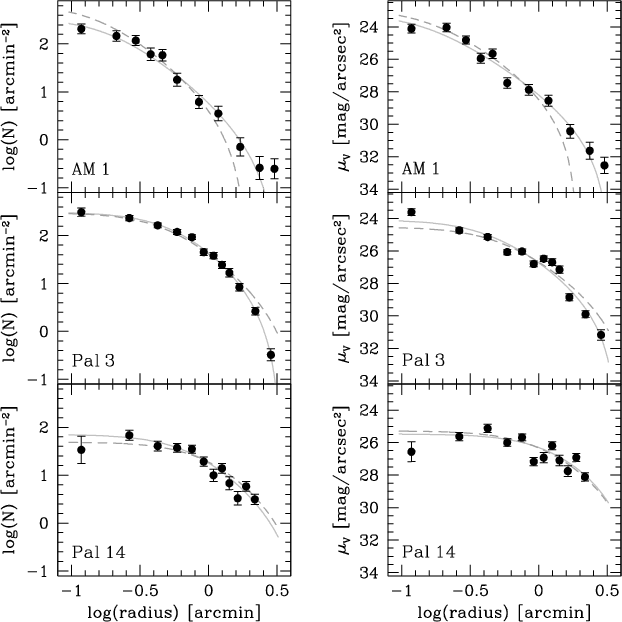
\includegraphics{figures/king-profiles.png}}
\end{center}

\begin{flushright}
Hilker (2005)
\end{flushright}

\vfill
\end{slide}


%------------------------------------------------------------------------------
\begin{slide}
\begin{center}
{\large \color{red} 
                  From $\rho$ to $f$  }
\end{center}

Given any functional form for $\rho(r)$ which is non-negative everywhere, it can be shown
that:
\eq{
	f(E) = \frac{1}{\sqrt{8}\pi^2} \frac{d}{dE} \int_E^0 d\Phi \frac{\rho'(\Phi)}{\sqrt{\Phi-E}} \label{eq:fE}
}
where $\rho'(Phi) = d\rho(\Phi)/d\Phi$ and $\rho(\Phi)$ can be obtained by solving
the Poisson equation and inverting (see BT \S~4, for details).

The above equation is useful in constructing isotropic models of spherical systems with
known density profiles (e.g., inferred from observations). In some cases,
these can be derived analytically (e.g., Jaffe 1983, or Henrquist 1990).

Generally, it can be solved numerically -- it's frequently used to set up
initial conditions for spherical systems in N-body calculations.

\vfill
\end{slide}

%------------------------------------------------------------------------------
\begin{slide}
\begin{center}
{\large \color{red} 
                  Comparison of various profiles  }
\end{center}

The profiles derived above supply us with convenient starting points for
building models of stellar systems (galaxies and globular clusters).

\begin{itemize}

\item {\bf Plummer} model has a finite density in the core, and falls 
of as $r^{-5}$. It matches globular clusters reasonably well.
\item {\bf King} model has a finite core density and outer radius, and is a
good description of globular clusters.
\item {\bf Hernquist \& Jaffe} models both fall of as $r^{-4}$ at large
radii, with different slopes in the core (Jaffe is steeper). This fall-off
at large radii is observed in elliptical galaxies, and theoretically well
motivated (violent relaxation; BT \S 4.10.2).

\end{itemize}

\vfill
\end{slide}


%------------------------------------------------------------------------------
\begin{slide}
\begin{center}
{\large \color{red} 
                  Comparison of various profiles  }
\end{center}

\begin{center}
\vskip -0.0in
\scalebox{0.85}{\hskip 0.0in 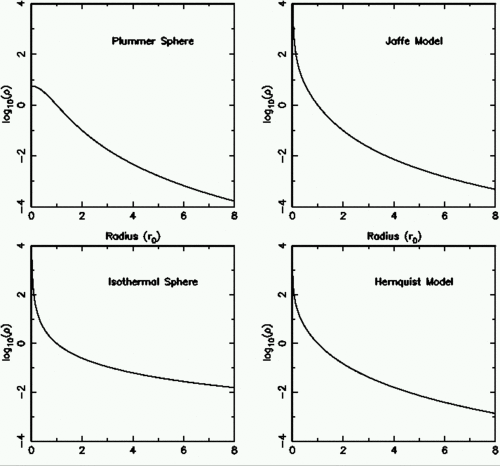
\includegraphics{figures/density_500.png}}
\end{center}

\begin{flushright}
\href{http://www.astro.utu.fi/~cflynn/galdyn/lecture4.html}{plot by Chris Flynn, Swinburne}
\end{flushright}

\vfill
\end{slide}


%------------------------------------------------------------------------------
\begin{slide}
\begin{center}
{\large \color{red} 
                  More about spherically symmetric profiles  }
\end{center}

Plummer, Jaffe and Hernquist are all realizations of a broader class of {\bf double
power-law} density profiles described by:
\eq{
	\rho(r) \propto \frac{1}{r^\gamma(1+r^{1/\alpha})^{(\beta - \gamma)\alpha}}
}
These behave as $\rho \propto r^{-\gamma}$ at $r \ll 1$ and $\rho \propto
r^{-\beta}$ at $r \gg 1$. Many of the well known density profiles fall into
this category:
\begin{center}
\vskip -0.5in
\scalebox{0.7}{\hskip 0.0in 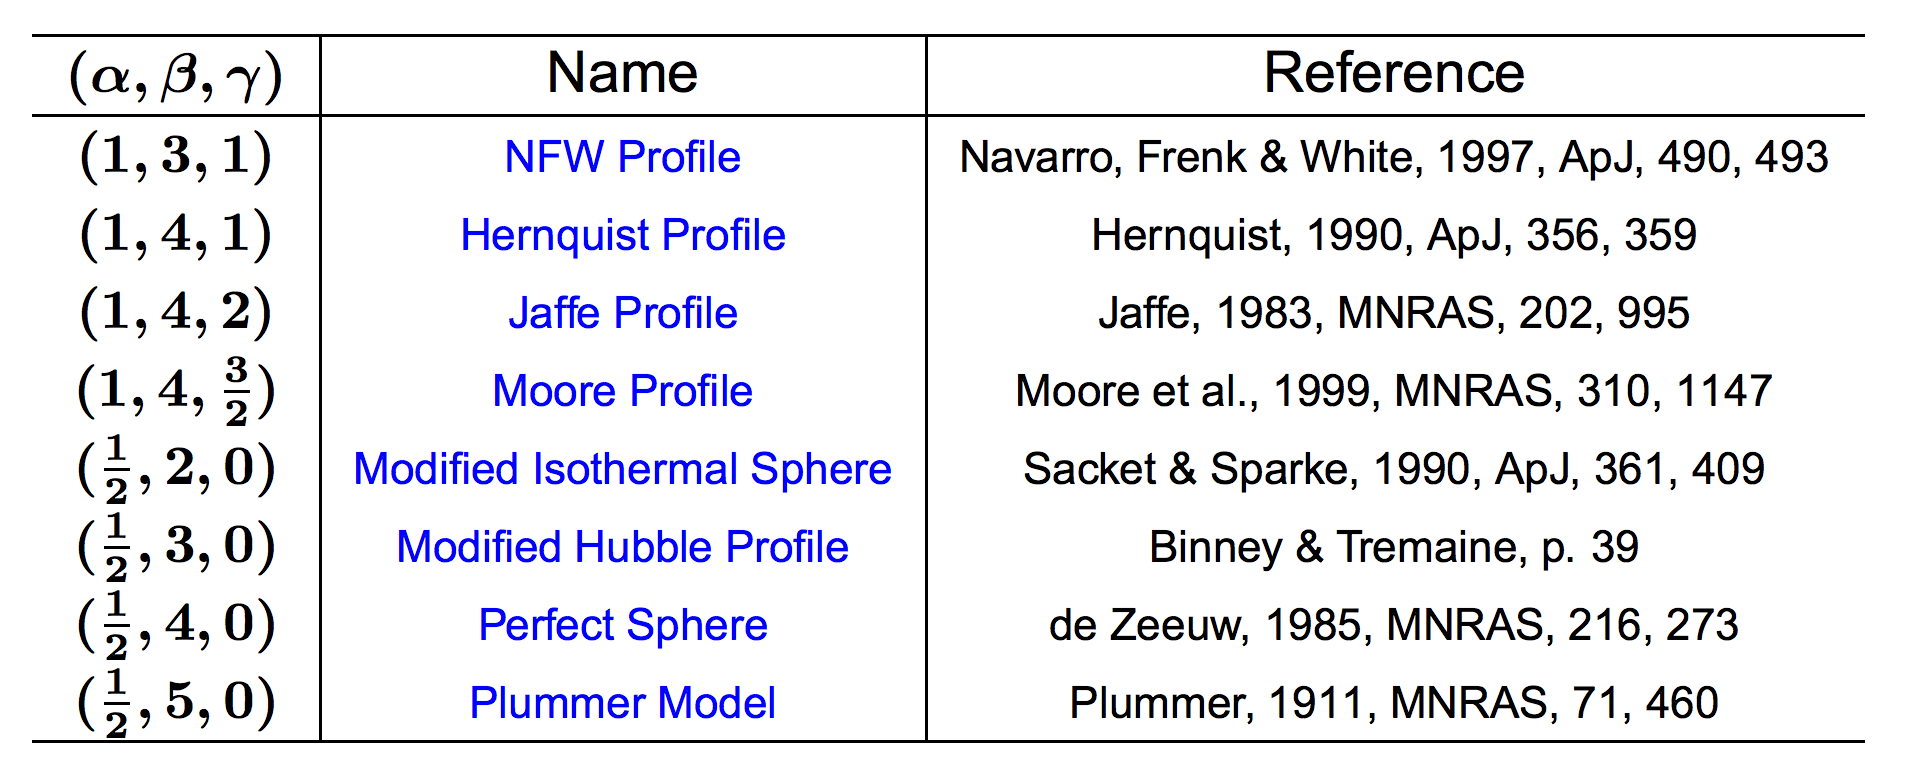
\includegraphics{figures/density-profiles-vdbosch.png}}
\end{center}
\begin{flushright}
\vskip -0.2in
Table from \href{http://www.astro.yale.edu/vdbosch/lecture2.pdf}{Frank van den Bosch, Yale}
\end{flushright}

\vfill
\end{slide}


%------------------------------------------------------------------------------
\begin{slide}
\begin{center}
{\large \color{red} 
                  Building Arbitrary Equilibrium Galaxies: Schwarzschild's Method  }
\end{center}

The examples given previously rely on our ability to derive closed-form
solutions to equations such as (\ref{eq:fE}).  Some of these solutions lead
to models that are useful in that they correspond to profiles seen in some
galaxies and globular clusters.

However useful that is, the analysis of the previous section does not give
us a general, {\em practical}, method to derive a steady-state distribution
function for an {\em arbitrary} distribution of density, $\rho(\b{x})$.

We'll now describe a semi-numerical technique due to Schwarzschild that
promises to do just that. It is commonly referred to as \b{Schwarzschild's method}
(Schwarzschild 1979).

\vfill
\end{slide}

%------------------------------------------------------------------------------
\begin{slide}
\begin{center}
{\large \color{red} 
                  Galaxy as a superposition of stars on orbits  }
\end{center}

A galaxy, as observed (as {\em imaged}) is nothing more than a superposition
of light coming from $\sim 10^{10}$ stars moving on orbits within its
potential.

If we imagine the orbits as {\em paths} along which stars traverse the galactic 
potential, we quickly see that some may be more frequented than others.
For example an orbit that takes a star around the center
of the Milky Way that's parallel to the plane of the disk is (roughly) $\sim
1000$~times more likely to have a star than an orbit perpendicular to it.

Schwarzschild's key insight was that if we developed a {\rm library} of all
(or approximately all) orbits that an observed density distribution admits, we could
try to construct a {\em superposition} that reproduces the observed density
$\rho(\b{x})$.

\vfill
\end{slide}

%------------------------------------------------------------------------------
\begin{slide}
\begin{center}
{\large \color{red} 
                  Schwarzschild's Method in a Nutshell }
\end{center}

\begin{enumerate}
\item Given $\rho(\b{x})$ find the potential $\Phi(\b{x})$.
\item Construct a large library of orbits admitted by $\Phi(\b{x})$
	\begin{itemize}
	\item Choose a large number ($N$) of initial conditions, each assigned to a particle.
	\item Integrate (numerically) each one of these over a long time $t \gg t_{\rm
	cross}$, tracing out its orbit.
	\item {\em Pixelize} each orbit onto a grid of $K$ cells, where the
		contribution of the orbit to each pixel will be proportional
		to the {\em time} a particle on the orbit spends in the pixel.
	\end{itemize}
\item Find a linear combination of orbits from the orbit library, each with
	non-negative weights, that reproduces $\rho(\b{x})$ when added
	together.
\end{enumerate}

\vfill
\end{slide}

%------------------------------------------------------------------------------
\begin{slide}
\begin{center}
{\large \color{red} 
                  Schwarzschild's Method: \#1. Density and potential  }
\end{center}

As the density distribution is known, the potential is obtained by solving
the Poisson equation:

\eq{
	\nabla^2 \Phi = - 4 \pi G \rho(\b{x})
}

No closed form solutions of this equation exist in general, but we can solve
it numerically on a finite grid.  For more, see the discussion of {\em
Poisson solvers} in BT \S2.9).

This gives us the potential $\Phi(\b{x})$ generated by the matter distribution
$\rho(\b{x})$, within which we can trace out the motions of test particles
(revealing their orbits).

\vfill
\end{slide}

%------------------------------------------------------------------------------
\begin{slide}
\begin{center}
{\large \color{red} 
                  Schw. Method: \#2. Construct the orbit library  }
\end{center}

Our next goal is to construct a {\em library} of all (at least in principle)
orbits that are possible in the derived potential.  We don't have to store
the actual orbits (i.e., $\b{x}(t)$ paths) into our library; what matters is
their {\em contribution to the observables}, typically, the density.

We therefore begin by {\bf gridding} the space occupied by the galaxy,
subdividing it into $K$ cells (voxels).  As our particle traverses the galaxy,
it will spend a varying amount of time $\delta t_j$ in each of our $K$
cells. Note that this includes $\delta t_j = 0$, i.e., some cells may never
be visited).

{\em The contribution to the observed density in each cell will be
proportional to the time the particle spends in the cell.}. We store these
contributions (in the most naive implementation, as a 3D data cube for each
orbit). The contribution to other observables (e.g., the LOSVD) could be
computed and stored as well.

\vfill
\end{slide}

%------------------------------------------------------------------------------
\begin{slide}
\begin{center}
{\large \color{red} 
                  Example: A regular non-resonant orbit in an axisymmetric potential. }
\end{center}

\begin{center}
\scalebox{0.55}{\hskip 0.0in 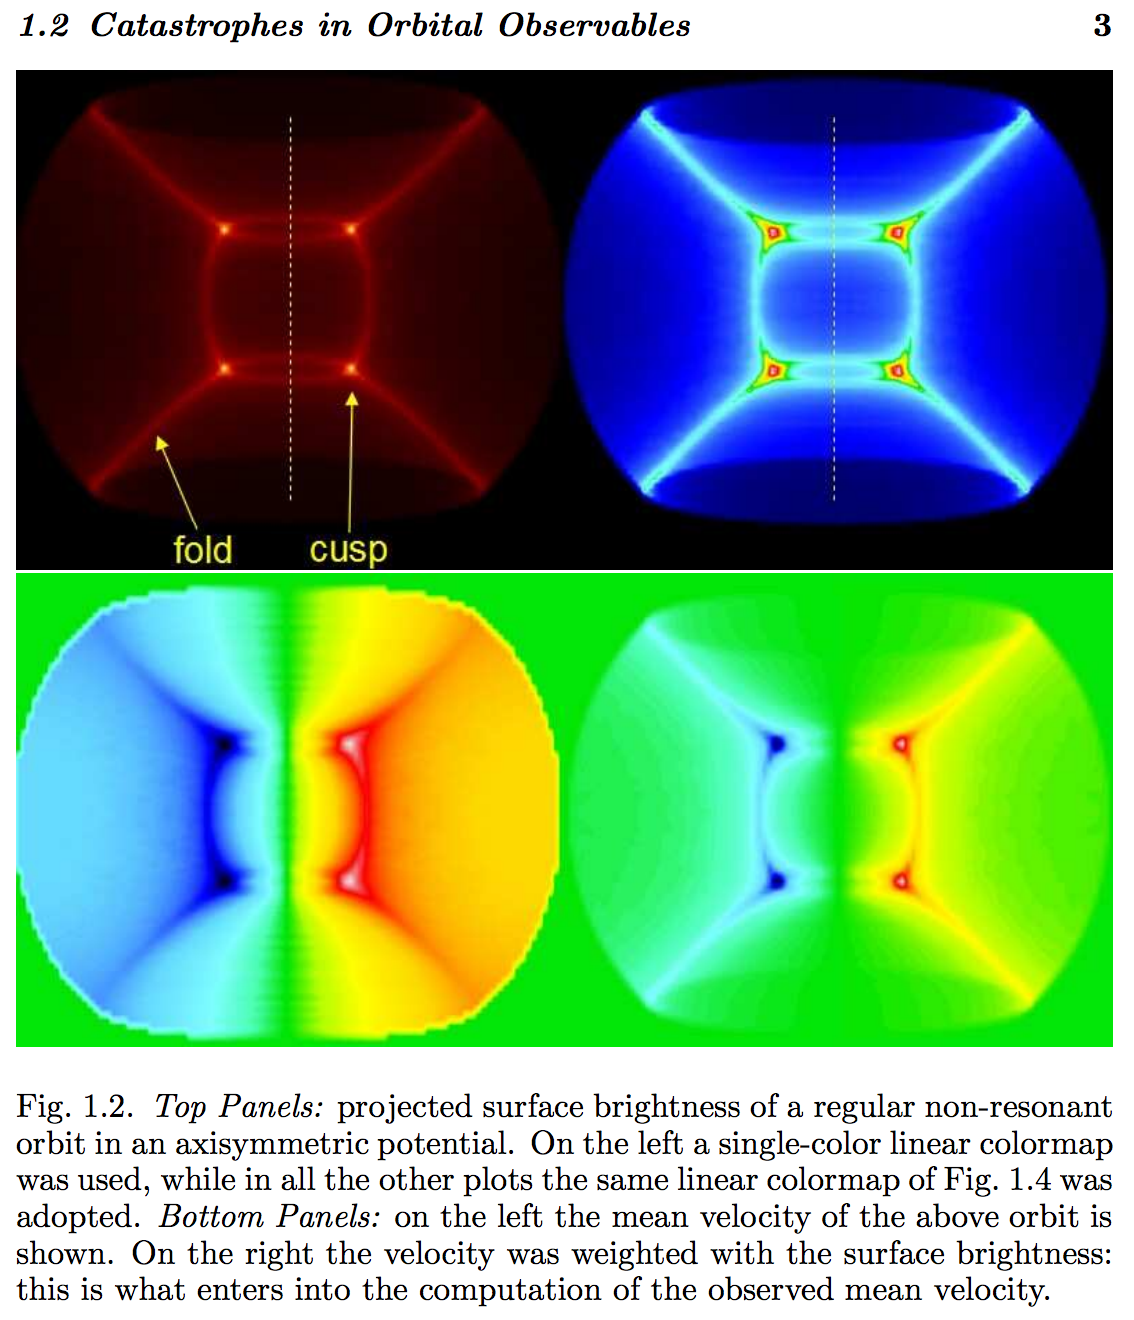
\includegraphics{figures/cappellari-catastrophes-axisymmetric.png}}
\end{center}

\begin{flushright}
Cappellari et al (2003); \href{https://arxiv.org/pdf/astro-ph/0302274v1.pdf}{astro-ph:0302274v1}
\end{flushright}

\vfill
\end{slide}

%------------------------------------------------------------------------------
\begin{slide}
\begin{center}
{\large \color{red} 
                  Example: A regular non-resonant orbit in a triaxial potential. }
\end{center}

\begin{center}
\vskip 0.5in
\scalebox{0.9}{\hskip 0.0in 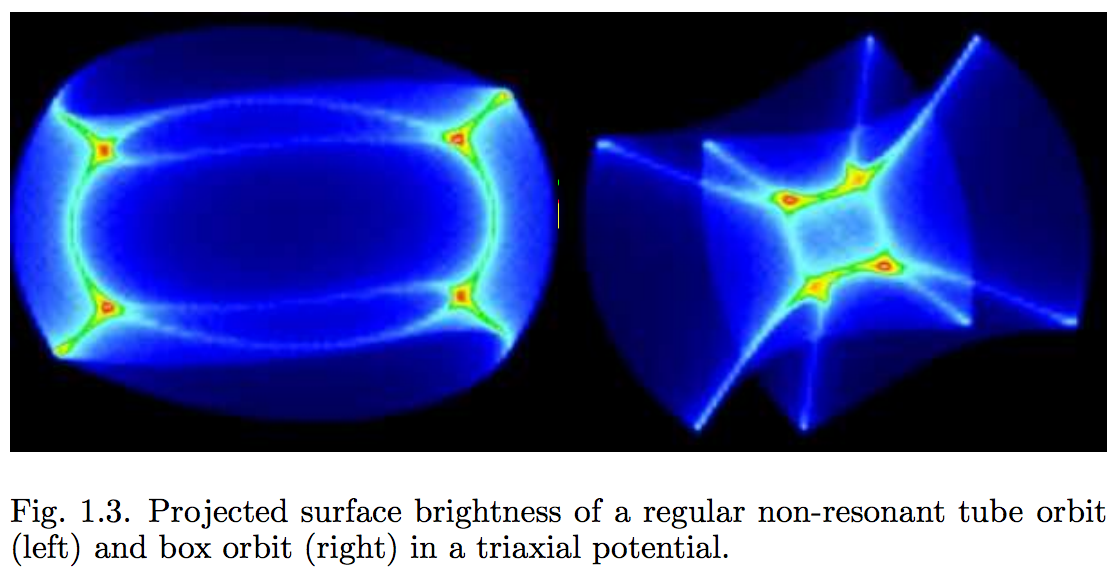
\includegraphics{figures/cappellari-catastrophes-triaxial.png}}
\vskip 0.5in
\end{center}

\begin{flushright}
Cappellari et al (2003); \href{https://arxiv.org/pdf/astro-ph/0302274v1.pdf}{astro-ph:0302274v1}
\end{flushright}

\vfill
\end{slide}

%------------------------------------------------------------------------------
\begin{slide}
\begin{center}
{\large \color{red} 
                  Schwarzschild's Method: \#3. Find a superposition that
corresponds to the observations  }
\end{center}

Let's assume the only observable we're trying to reproduce is the density,
$\rho(\b{x})$. The contribution to cell $j$ of volume $V_j$ is equal to:
\eq{
	m_{j} = \rho(\b{x_{j}}) V_{j}
}.
Let us assume that each orbit in our library is populated by a large number
of stars, uniformly distributed in orbital phase, and that the total mass of
stars on orbit $i$ is $w_i M$, were $w_i$ is the weight, and $M$ is the
total mass of the galaxy. Therefore, the mass in cell $j$ will be equal to
the sum of the contributions from orbits that cross it, or:
\eq{
	m_{j,{\rm constructed}} = M \sum_{i=1}^{N} w_i p_{ij}
}

\vfill
\end{slide}

%------------------------------------------------------------------------------
\begin{slide}
\begin{center}
{\large \color{red} 
                  Schwarzschild's Method: \#3. Find a superposition that
corresponds to the observations  }
\end{center}

Therefore, we're looking for a solution of:
\eq{
	0 = \Delta_j \equiv m_j - M \sum_{i=1}^{N} w_i p_{ij} \label{eq:sch}
}.

This is a set of $K$ linear equations for the $N$ unknown weights $w_i$. 
Note that the condition that $\sum_j m_j = M$ implies that $\sum_j w_j = 1$.

In principle, by choosing $N = K$ would make it possible to trivially solve
this sytem; however, for the model to be physical, all $w_i$ have to be
positive. In practice, this choice leads to some values of $w_i$ being
negative.

\vfill
\end{slide}

%------------------------------------------------------------------------------
\begin{slide}
\begin{center}
{\large \color{red} 
                  Schwarzschild's Method: \#3. Find a superposition that
corresponds to the observations  }
\end{center}

The way we work around this problem is to take $N \gg K$, i.e., we observe
many more orbits than spatial cells. In that case, the points that satisfy
the equations form an ($N - K$) dimensional subspace of the $N$ dimensional
space of weight vectors $\b{w}$.

A physically meaningful solution exists if this subspace passes through the
region where all $w_i > 0$. It's possible there are no solutions -- i.e.,
the input $\rho(x)$ cannot be explained as a steady-state self-gravitating
system.

But note that if a solution exists, there will {\bf generally be {\em infinitely
many} solutions $\b{w}$}. Every one corresponds to an acceptable galaxy
model.

\vfill
\end{slide}

%------------------------------------------------------------------------------
\begin{slide}
\begin{center}
{\large \color{red} 
                  The Objective Function  }
\end{center}

That is, {\bf we either find no solution, or an infinite set of possible
solutions}.

We must bring additional information to the table, introduce {\em additional
constraints} to narrow down the set of acceptable solutions, perhaps even
down to a single one.  This is normally done by choosing the solution that
maximizes some {\bf objective function $\phi(\b{w})$}.

A simple choice is one where $\phi(\b{w})$ is linear:
\eq{
	\phi(\b{w}) = \sum_i \phi_i w_i
}
Solving the system (\ref{eq:sch}) under these constraints is an exercise in
a mathematical optimization technique called {\bf linear programming}. See
\url{http://www.math.ucla.edu/~tom/LP.pdf} for a consise introduction.

\vfill
\end{slide}

%------------------------------------------------------------------------------
\begin{slide}
\begin{center}
{\large \color{red} 
                  Choosing the Objective Function  }
\end{center}

The {\bf objective function} is how we impose additional constraints (that is,
{\bf import additional knowledge about the system}) into the modeling procedure.

While linear objective function is straightforward to write and apply, it is
not optimal. For one, it's not obvious how to physically motivate the maximization
of some linear function of the weights. Schwarzschild himself pretty much
picked his $\phi_i$ at random, though his goal was to prove that there {\em
exist} self-consistent models of triaxial galaxies. There are also other,
more technical reasons, why a linear $\phi(\b{w})$ is not optimal (see BT
for details).

Other options: maximizing the entropy, $\phi(\b{w}) = S \equiv -\sum_i w_i
\ln w_i$ (see BT~\S4.10.1), or a quadratic objective function of the form
$\phi(\b{w}) = - \sum_i w_i^2/W_i$ where $W_i > 0$. Solving with the latter is an
exercize in {\bf quadratic programming}; the physical meaning is to find the
values of $w_i$ that are closest to $W_i$ while satisfying $\rho(\b{x})$. 
Into $W_i$ we can encode any priors we have on the expected orbital
structure of the galaxy being studied.

\vfill
\end{slide}

%------------------------------------------------------------------------------
\begin{slide}
\begin{center}
{\large \color{red} 
                  Extensions of Schwarzschild's Method }
\end{center}

A particularly fruitful extension of Schwarzschild's method is to model
kinematic data (e.g., such as those coming from integral field units).

These observations result in measurements of LSOVD at pixels within the
galaxies' footprints, and the LOSVD at each point is a linear function of
the orbit weights, $w_i$. So the function to {\em minimize} to is simply
$\chi^2$.

In other words, $\phi(\b{w}) = - \chi^2$. This can be solved using quadratic
programming techniques. It has been applied to the understanding of dynamics
of early type galaxies, as well as the search for central black holes.

\vfill
\end{slide}

%------------------------------------------------------------------------------
\begin{slide}
\begin{center}
{\large \color{red} 
                  Schwarzschild's Method: Building an ETG constrained by IFU observations   }
\end{center}

\begin{center}
\vskip 1.0in
\scalebox{1.4}{\hskip 0.0in 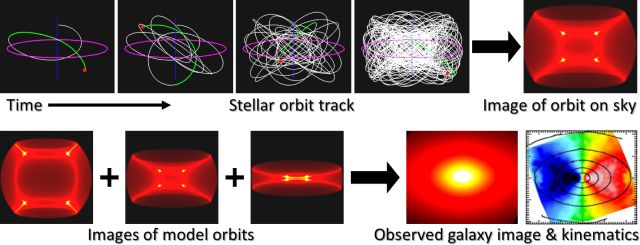
\includegraphics{figures/Schwarzschild_Modelling.jpg}}
\vskip 1.0in
\end{center}

\begin{flushright}
Cappellari (2015); \url{http://adsabs.harvard.edu/abs/2014arXiv1410.7329C}
\end{flushright}

\vfill
\end{slide}

%------------------------------------------------------------------------------
\begin{slide}
\begin{center}
{\large \color{red} 
                  Applications of Schwarzschild Modelling   }
\end{center}

Schwarzschild modelling has been successfuly applied to a variety of topics.
Two more recent ones:
\begin{itemize}
\item Search for massive black holes at the centers of galaxies 
(e.g., Richtone \& Tremaine 1985; van der Marel et al. 1998;
Gebhardt et al. 2003), leading to the discovery of $M-\sigma$ relation.
\item Modeling of the large-scale dynamics of early type galaxies
(e.g., Capellari et al. 2006), constraining the mass densities and orbital
structure.
\end{itemize}

\vfill
\end{slide}

%------------------------------------------------------------------------------
\begin{slide}
\begin{center}
{\large \color{red} 
                  The Importance of a Good Orbit Library  }
\end{center}

It's important that the orbit library is fairly complete, i.e., that it
combines a sufficiently wide variety of types of orbits, with a reasonably
dense sampling of the phase space:

\begin{itemize}
\item If this is not the case, there may not be even a single solution to
the constraint equaton (\ref{eq:sch}) with non-negative weights and secondly,
\item we often wish to explore a full set of allowable models, to understand
better understand the limitations and the constraining power of our dataset.
\end{itemize}

In practice, generating a good orbit library requires some intuition and
experience. This part is as much art as science.

\vfill
\end{slide}


\end{document}


